%
%	Praxisbezug
%

\pagebreak
\section{CIS Scans}

\onehalfspacing

\subsection{CIS Benchmarks for Kubernetes}

In the previous chapter, we've covered the necessary mechanism to codify and enforce standards for our Kubernetai across our IT organization, using Terraform and Rancher templates. Now let's move one step further and look at checking our clusters for security issues.

There are many security standards and recommendations for IT, but there is one organization that's universally recognized as leading the field of IT security and compliance: The Center for Internet Security, Inc. (CIS\textsuperscript{\textregistered})

CIS is a community-driven nonprofit and responsible for CIS Controls\textsuperscript{\textregistered} and CIS Benchmarks \texttrademark, which are globally recognized as the best practices for securing IT systems and data. If you want to look at the actual CIS Benchmarks, they are available for download on the CIS website; you'll need to register with CIS first, though.

Testing a platform against a CIS Benchmark is usually a lengthy process. Fortunately, there are several automated scan tools available for Kubernetes, and with Rancher 2.4, a CIS Scan is now available for all managed Clusters right from the Rancher GUI.

CIS Scans can be invoked manually or scheduled regularly, with Rancher's Alert Manager reporting it. With Terraform provider version 1.8.0 (March 2020), this feature is now also available in Terraform, too.\footnote{See \textit{Rancher Labs (2020)}: Changelog. \cite{ChangeLog}}

\subsection{CIS Scan GUI}

In the classic GUI, at the cluster level, Rancher offers two choices of CIS Scans:

\begin{itemize}
\item RKE-CIS-1.4 Permissive
\item RKE-CIS-1.4 Hardened
\end{itemize}

Both scans are based on the Kubernetes CIS Benchmark version 1.4, with different sets of enabled controls adapted by Rancher to the underlying Rancher Kubernetes Engine (RKE). A default installation will pass the permissive profile tests. To pass the hardened profile, you'll need to adhere fully to the Rancher 2.3 Hardening guide.\footnote{See \textit{Rancher Labs (2019)}: Hardening Guide. \cite{hardeningGuide}}

The cluster we created in the previous chapter is using mostly default values and thus does not pass the scan with the hardened profile:

\begin{figure}[H]
\centering
\caption {CIS Scan GUI}
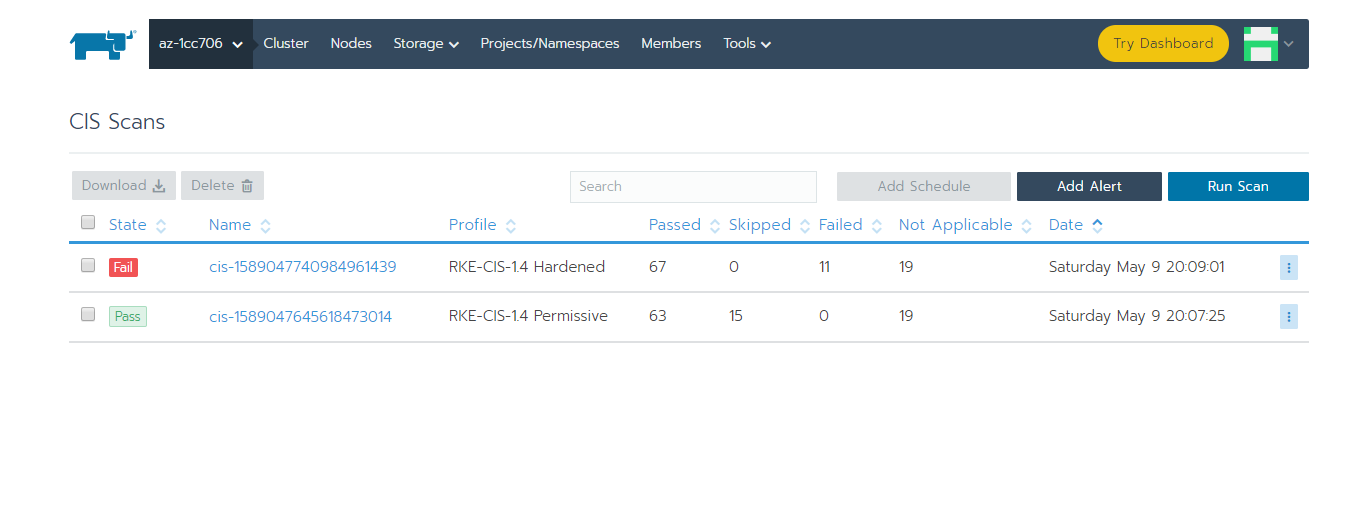
\includegraphics[width=\linewidth]{images/cis-scan-overview.png}
\label{fig:cisScanOverview}
\end{figure}

\subsection{Hardened CIS Scan}

We will not go through all hardening steps in detail, but look at one control as an example:

\begin{figure}[H]
\centering
\caption {Hardened CIS Scan}
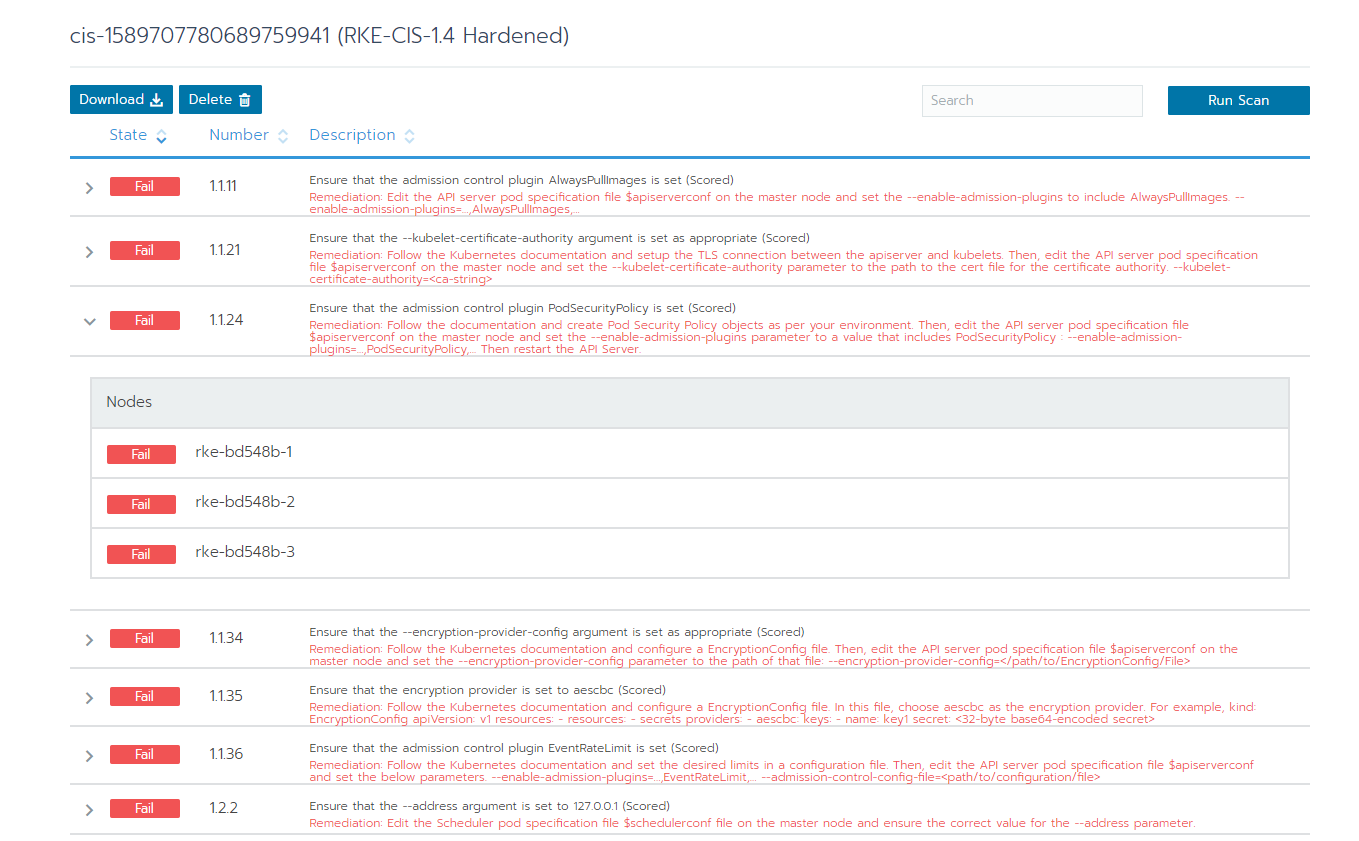
\includegraphics[width=\linewidth]{images/cis-scan-fail.png}
\label{fig:cisScanFail}
\end{figure}

The control we'll be focusing on is 1.1.24: Ensure that the admission control plugin PodSecurityPolicy is set.

To fully harden your cluster, please follow the hardening instructions mentioned above; for now, we'll look at the missing Pod Security Policy.

\subsection{Kubernetes Security Policies}

What is a Pod Security Policy (PSP)? Kubernetes provides two types of security policies, one for pod security and one for network security. Pod security policies, as the name implies, govern security-relevant aspects of pod specification,\footnote{See \textit{The Linux Foundation (2019)}: Pod Security Policies. \cite{podSecurity}}, whereas network policies govern the allowed communication between groups of pods and the outside world.\footnote{See \textit{The Linux Foundation (2019)}: Network Policies. \cite{netSecurity}}

It is good practice when running a Kubernetes cluster in production to secure access with Pod Security Policies.\footnote{See \textit{Price, J. (2020)}: Kubernetes - Pod Security Policies. \cite{examplePsp}} Rancher offers two pre-built PSPs (named "restricted" and "unrestricted") and a GUI to create your own.\footnote{See \textit{Iradier, A. (2020)}: Enhancing Kubernetes Security with Pod Security Policies. \cite{detailPsp}}

There are many controls within a Pod Security Policy that we won't cover in this document; instead, we'll focus on the admission controller.

\subsection{Remediation}

The scan gives us the following remediation instruction:

\begin{verbatim}
Remediation: Follow the documentation and create Pod 
Security Policy objects as per your environment   
\end{verbatim}

To mitigate the failed control, what we need to do is to add a default Pod Security Policy. Fortunately, that's relatively easy in Rancher. In the cluster template, we need to enable PSP support and define the default policy.

We can do that by adding the following line to our template definition in Terraform:

\begin{lstlisting}[caption=Cluster Template with PSP, frame=single, basicstyle=\ttfamily]
default_pod_security_policy_template_id = "restricted"
\end{lstlisting}

Or, if your prefer the Rancher GUI, you can set the default Pod Security Policy there too:

\begin{figure}[H]
\centering
\caption {Rancher PSP Support}
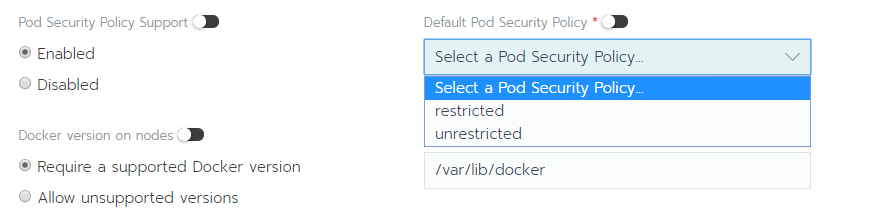
\includegraphics[width=\linewidth]{images/rancher-psp-support.png}
\label{fig:rancherPSP}
\end{figure}

Once you've enabled the PSP, the control will pass in the CIS scan. It's an iterative process: Based on your IT organization's needs, you'll have to identify the controls critical for your business and implement the remediation steps one by one, as needed, to harden your cluster.

Automated CIS scans will then give you a valuable tool to check all your Kubernetai regularly for security issues and regulatory compliance, and help you to act on issues accordingly.
